\documentclass[12pt,a4]{article}




\usepackage{graphicx,amsmath,amssymb,amsthm, boxedminipage,xcolor,amscd,amsbsy,latexsym,url,bm}

%\usepackage[lined,boxed]{algorithm2e}

\usepackage{algorithm}
\usepackage{algpseudocode}


\newtheorem{theorem}{Theorem}[section]
\newtheorem{proposition}[theorem]{Proposition}
\newtheorem{lemma}[theorem]{Lemma}
\newtheorem{corollary}[theorem]{Corollary}
\newtheorem{definition}[theorem]{Definition}

\newtheorem*{theorem*}{Theorem}
\newtheorem*{lemma*}{Lemma}
\newtheorem*{solution}{Solution}
\newtheorem*{proposition*}{Proposition}


\newtheorem{exercise}[theorem]{Exercise}
\newtheorem{exerciseD}[theorem]{*Exercise}
\newtheorem{exerciseDD}[theorem]{**Exercise}

\let\oldexercise\exercise
\renewcommand{\exercise}{\oldexercise\normalfont}

\let\oldexerciseD\exerciseD
\renewcommand{\exerciseD}{\oldexerciseD\normalfont}

%\let\oldexerciseD\exerciseD
%\renewcommand{\exerciseD}{\oldexerciseD\normalfont}

%\let\oldexerciseDD\exerciseDD
%\renewcommand{\exerciseDD}{\oldexerciseDD\normalfont}

\newcommand{\E}{\mathbb{E}}
%\newcommand{\nth}[1]{#1^{\textsuperscript{th}}}
\newcommand{\scalar}[2]{\ensuremath{\langle #1, #2\rangle}}
\newcommand{\floor}[1]{\left\lfloor #1 \right\rfloor}
\newcommand{\ceil}[1]{\left\lceil #1 \right\rceil}
\newcommand{\norm}[1]{\|#1\|}
\newcommand{\pfrac}[2]{\left(\frac{#1}{#2}\right)}
\newcommand{\nth}[1]{#1^{\textsuperscript{th}}}
\newcommand{\core}{\textnormal{core}}



\newif\ifsolution

\solutionfalse

\newcommand{\answer}[1]{
\ifsolution
{\color{blue} #1}
\else
\fi
}



\newcommand{\poly}{\textnormal{poly}}
\newcommand{\quasipol}{\textnormal{quasipol}}
\newcommand{\ssubexp}{\textnormal{stronglySubExp}}
\newcommand{\wsubexp}{\textnormal{weaklySubExp}}
\newcommand{\simplyexp}{\textnormal{E}}
\newcommand{\expo}{\textnormal{Exp}}



\newcommand{\N}{\mathbb{N}}
\newcommand{\nn}{\mathbb{N}_0^n}
\newcommand{\R}{\mathbb{R}}
\newcommand{\Z}{\mathbb{Z}}


\definecolor{darkgreen}{rgb}{0,0.6,0}

\date{}

\title{
\hbox{  Mathematical Foundations of Computer Science}
  \vspace{3mm}
{\normalsize CS 499,	Shanghai Jiaotong University,  Dominik Scheder\\
%\vspace{3mm}
Spring 2019}
}


\begin{document}

\maketitle

%\begin{quotation}
%  You are welcome to discuss the exercises in the discussion
%  forum. Please take them serious. Doing the exercises is as important
%  than watching the videos.
%
%  I intentionally included very challenging exercises and marked them
%  with one or two ``$*$''. No star means you should be able to solve
%  the exercises without big problems once you have understood
%  the material from the video lecture. One star means it requires 
%  significant additional thinking. Two stars means it is not 
%  unlikely that you will fail to solve them, even once you have understood
%  the material and thought a lot about the exercise. Don't feel bad
%  if you fail. Failure is part of learning.
%
%  This is the first time this course is online. Thus there might be mistakes
%  (typos or more serious conceptual mistakes) in the exercises. I will be 
%  grateful if you point them out to me!
%\end{quotation}

\begin{document}

\maketitle
\newcommand{\val}{\textnormal{val}}


\setcounter{section}{10}

\section{Matchings and Network Flow}



\begin{itemize}
 \item Homework assignment published on Thursday, 2019-05-23.
 \item Submit questions and first solutions by Wednesday, 2019-05-29, 12:00.
 \item Submit final solution by Wednesday, 2019-06-05.
\end{itemize}


\subsection{Matchings}


Consider the Hamming cube $\{0,1\}^n$. We can view it as a graph $H_n$, 
where the vertex set is $\{0,1\}^n$ and two vertices $x,y$ are connected by an 
edge if $x$ and $y$ differ in exactly one coordinate.
Define the $\nth{k}$ layer to be 
$L_k := \{ x \in \{0,1\}^n \ | \ |x|_1 = k\}$, where $|x|_1$ denotes the number of $1$s 
in $x$. Note that the subgraph induced by layer $k$ and layer $k+1$ is a bipartite 
graph $H_n [ L_k \cup L_{k+1}]$. See the picture below for an illustration ($n=3, k=1$):
\begin{center}
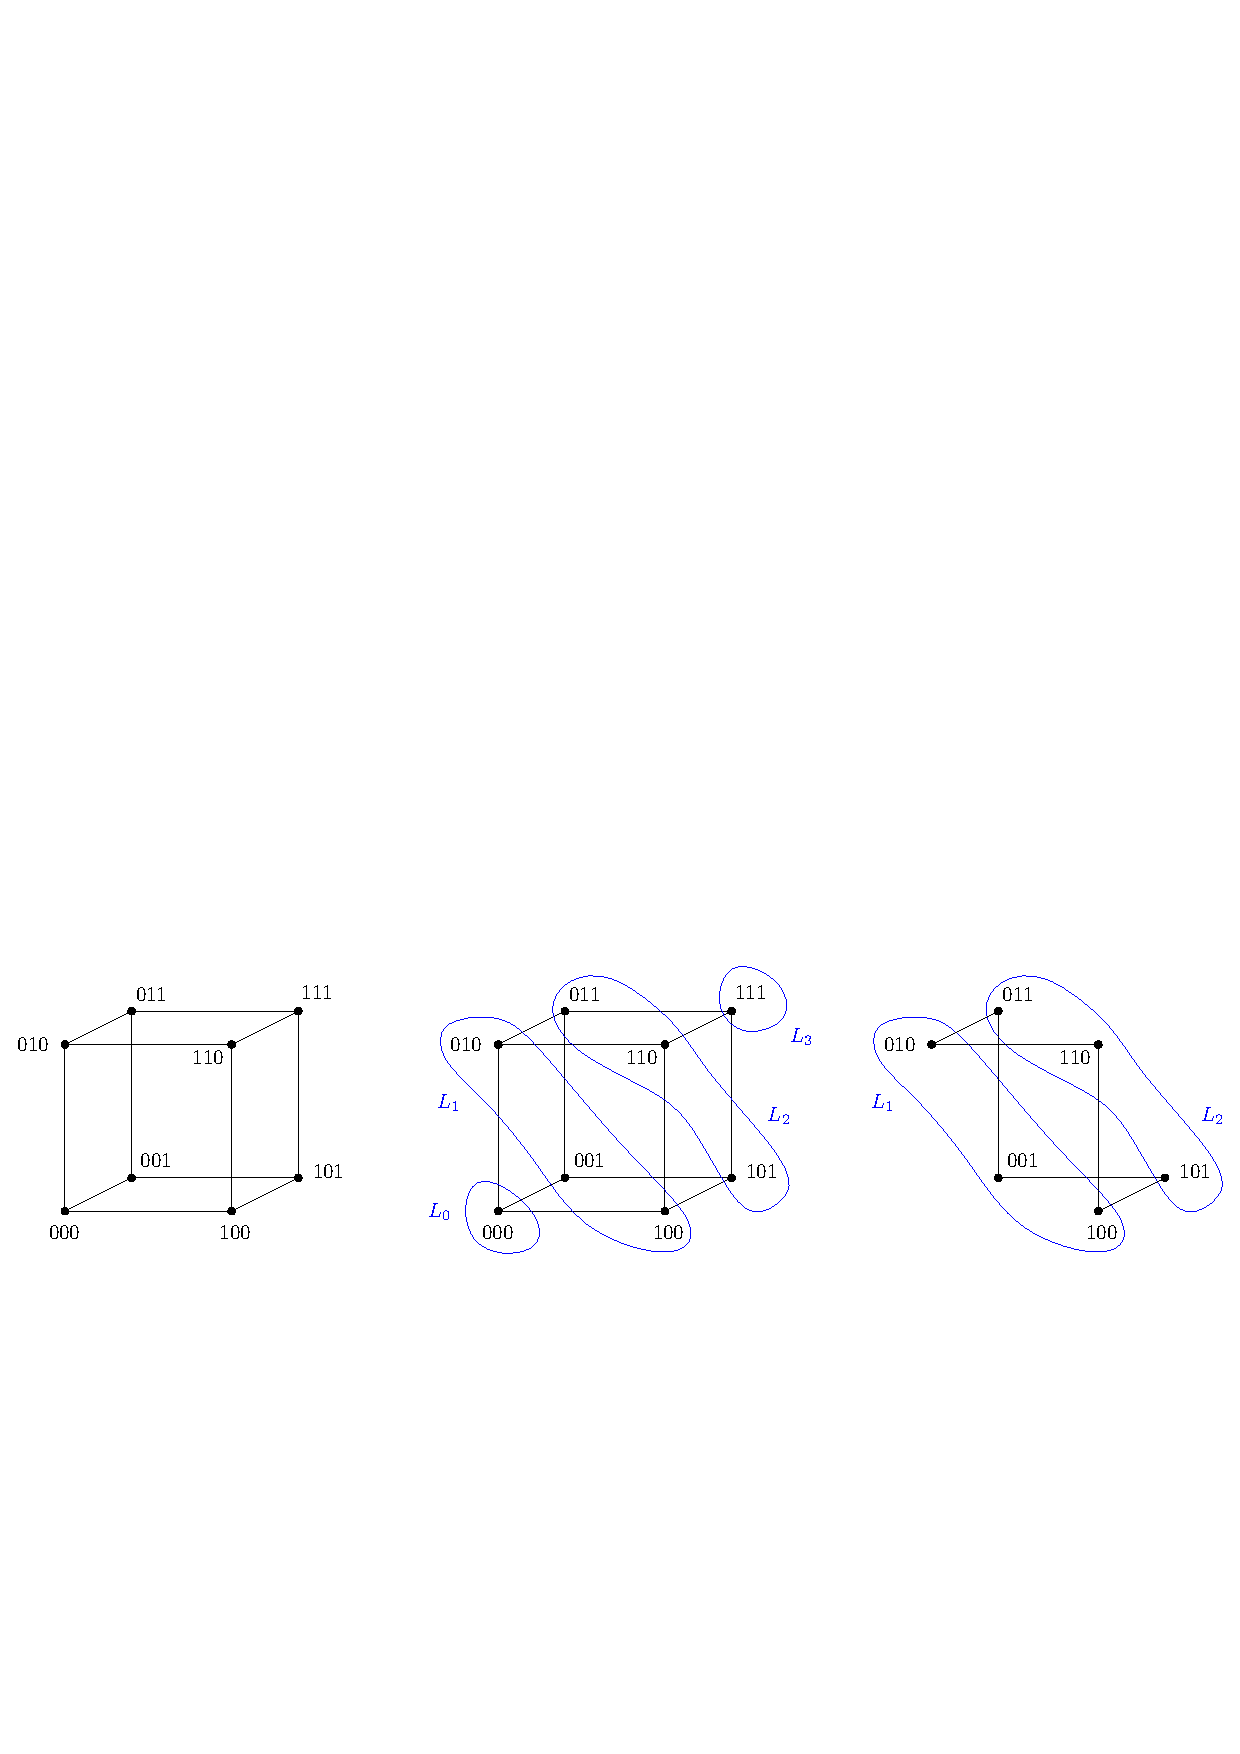
\includegraphics[width=\textwidth]{figures/hamming-cube-layer-graph.pdf}
\end{center}
\begin{exercise}
 Let $0 \leq k < n/2$.
 Show that the bipartite graph $H_n [L_k \cup L_{k+1}]$ has a matching of size $|L_k| = {n \choose k}$.
\end{exercise}

\textbf{Solution.} Degree of each vertex in $L_k$ is $n-k$, and vertex in $L_{k+1}$ is $k+1$. Because $0 \leq k < n/2$, then $n-k\geq k+1$. Also, for arbitrary  two vertices in $L_k$, there is no overlap between edges that these two vertices can cover. By deleting a vertex in $L_{k}$, we always cover the maximal possible number of the remaining edges. Therefore, the minimum vertex cover is $L_k$. According to Konig Theorem, matching size is $|L_k|$.

\begin{exercise}
 Let $G = (V,E)$ be a bipartite graph with left side $L$ and right side $R$.
 Suppose $G$ is $d$-regular (every vertex has degree $d$), so in particular $|L| = |R|$.
 Show that $G$ 
 has a perfect matching (that is, a matching $M$ of size $|L|$).
\end{exercise}

\textbf{Solution.} Degree of each vertex is $d$.  For arbitrary  two vertices in $L_k$, there is no overlap between edges that these two vertices can cover. Consider the vertex cover problem, by always deleting a vertex in $L$ (or $R$), we cover the maximal possible number of the remaining edges. Therefore, $L$ and $R$ are minimum vertex cover. According to Konig Theorem, maximum matching size is $|L|$. So we can find a matching of size $|L|$.


\begin{exercise}
  Let $G$ a $d$-regular bipartite graph. Show that the edges $E(G)$ can be partitioned
  into $d$ perfect matchings. That is, there are matchings $M_1, \dots, M_d \subseteq E(G)$ such that
  (1) $M_i \cap M_j = \emptyset$ for $1 \leq i < j \leq d$ and 
  (2) $M_1 \cup M_2 \cup \dots \cup M_d = E(G)$.
\end{exercise}

\textbf{Solution.} According to Exercise 11.2, we can find a perfect matching in a $d$-regular bipartite graph. After delete this perfect matching, the graph becomes a $(d-1)$-regular bipartite graph, where we can find another perfect matching. We keep doing this until there is no edge in the graph. Therefore, the edges $E(G)$ can be partitioned into $d$ perfect matchings.

\subsection{Networks with Vertex Capacities}

Suppose we have a directed graph $G = (V,E)$ but instead of 
{\em edge capacities} we have {\em vertex capacities} $c: V \rightarrow \R$.
Now a flow $f$ should observe the {\em vertex capacity constraints}, i.e.,
the outflow from a vertex $u$ should not exceed $c(u)$:
\begin{align*}
  \forall u \in V: \sum_{v \in V, f(u,v) > 0} f(u,v) \leq c(u) \ .
\end{align*}

\begin{exercise} Consider networks with vertex capacities.
  \begin{enumerate}
    \item Show how to model networks with vertex capacities by 
      networks with edge capacities. More precisely, 
      show how to transform $G = (V,E,c)$ with $c: V \rightarrow \R^+$
      into a network $G' = (V',E',c')$ with $c': E' \rightarrow \R^+$
      such that every $s$-$t$-flow $f$ in $G$ that respects the vertex capacities 
      corresponds to an $s$-$t$-flow $f'$ (of same value) in $G'$ that
      respects edge capacities, and vice versa.
    \item Draw a picture illustrating your solution.
    \item Show that there is a polynomial time algorithm solving the
      following problem: Given a directed graph $G = (V,E)$ and two
      vertices $s,t \in V$.  Are there $k$ paths $p_1,\dots,p_k$, each
      from $s$ to $t$, such that the paths are {\em internally vertex
        disjoint}?  Here, internally vertex disjoint means that for $i
      \ne j$ the paths $p_i,p_j$ share no vertices besides $s$ and
      $t$.
  \end{enumerate}
\end{exercise}
\textbf{Solution.}
\begin{enumerate}
  \item Transform $G$ into $G'$ in the following steps:
  \begin{enumerate}
    \item For each $v\in V$, split it into two vertices, $v_{in}$ and $v_{out}$. Add them into $V'$. Add an edge $(v_{in},v_{out})$ with capacity $c(v)$ into $E'$.
    \item For each $(u,v)\in E$, add $(u_{out},v_{in})$ with  capacity $\infty$ into $E'$.
  \end{enumerate}
  Then the transformation is complete. Next we prove that every $s$-$t$-flow $f$ in $G$ corresponds to an $s$-$t$-flow $f'$ of same value in $G'$.

  \textbf{Proof.} ``$\Leftarrow$'':An $s$-$t$-flow $f:V\times V\rightarrow \mathbb{R}$ in $G$ satisfies that
  \begin{align*}
    \forall u\in V,\quad &\sum_{(u,v)\in E}f(u,v)\leq c(u)\\
    f(u,v)=-f(v,u) \quad&(f(u,v)>0\;\; \text{if} \;\;(u,v)\in E)\\
    \sum_{v\in V}f(u,v)&=0,\; \forall u\in V\setminus \{s,t\}
  \end{align*}
  For corresponding $f'$, we only need to show the capacity constraint is satisfied as the other two constraints are just copied as they have the same value. Combine two of the constraints together we have 
  \begin{align*}
    f'(u_{in},u_{out})=\sum_{(v_{out},u_{in})\in E'}f'(v_{out},u_{in})=\sum_{(v,u)\in E}f(v,u)=\sum_{(u,v)\in E}f(u,v)\leq c(u)=c'(u_{in},u_{out})
  \end{align*}
  
 
  And for other edges in $E'$, it is trivial to show $f'(u,v)\leq c'(u,v)=\infty$.

  Therefore the corresponding $f':V'\times V'\rightarrow \mathbb{R}$ in $G'$ satisfies that $\forall u,v\in V'$, $f'(u,v)\leq c'(u,v)$, which is indeed a flow w.r.t edge capacities.

  ``$\Rightarrow$'':An $s$-$t$-flow $f':V'\times V'\rightarrow \mathbb{R}$ in $G'$ satisfies that
  \begin{align*}
    \forall u,v\in V',\quad &f'(u,v)\leq c'(u,v)\\
    f'(u,v)=-f'(v,u) \quad&(f'(u,v)>0\;\; \text{if} \;\;(u,v)\in E')\\
    \sum_{v\in V'}f'(u,v)&=0,\; \forall u\in V'\setminus \{s,t\}
  \end{align*}
  Likewise, we only need to show the corresponding $f:V\times V\rightarrow \mathbb{R}$ in $G$ satisfies the capacity constraint. Actually we have
  \begin{align*}
    \sum_{(u,v)\in E}f(u,v)=\sum_{(u_{out},v_{in})\in E'}f'(u_{out},v_{in})=f'(u_{in},u_{out})\leq c'(u_{in},u_{out})=c(u)
  \end{align*}
  Therefore $f$ is a flow w.r.t vertex capacities.\qed
  
  \item Figure~\ref{fig-transform} shows an example of the transform.
  \begin{figure}[ht]
    \centering
    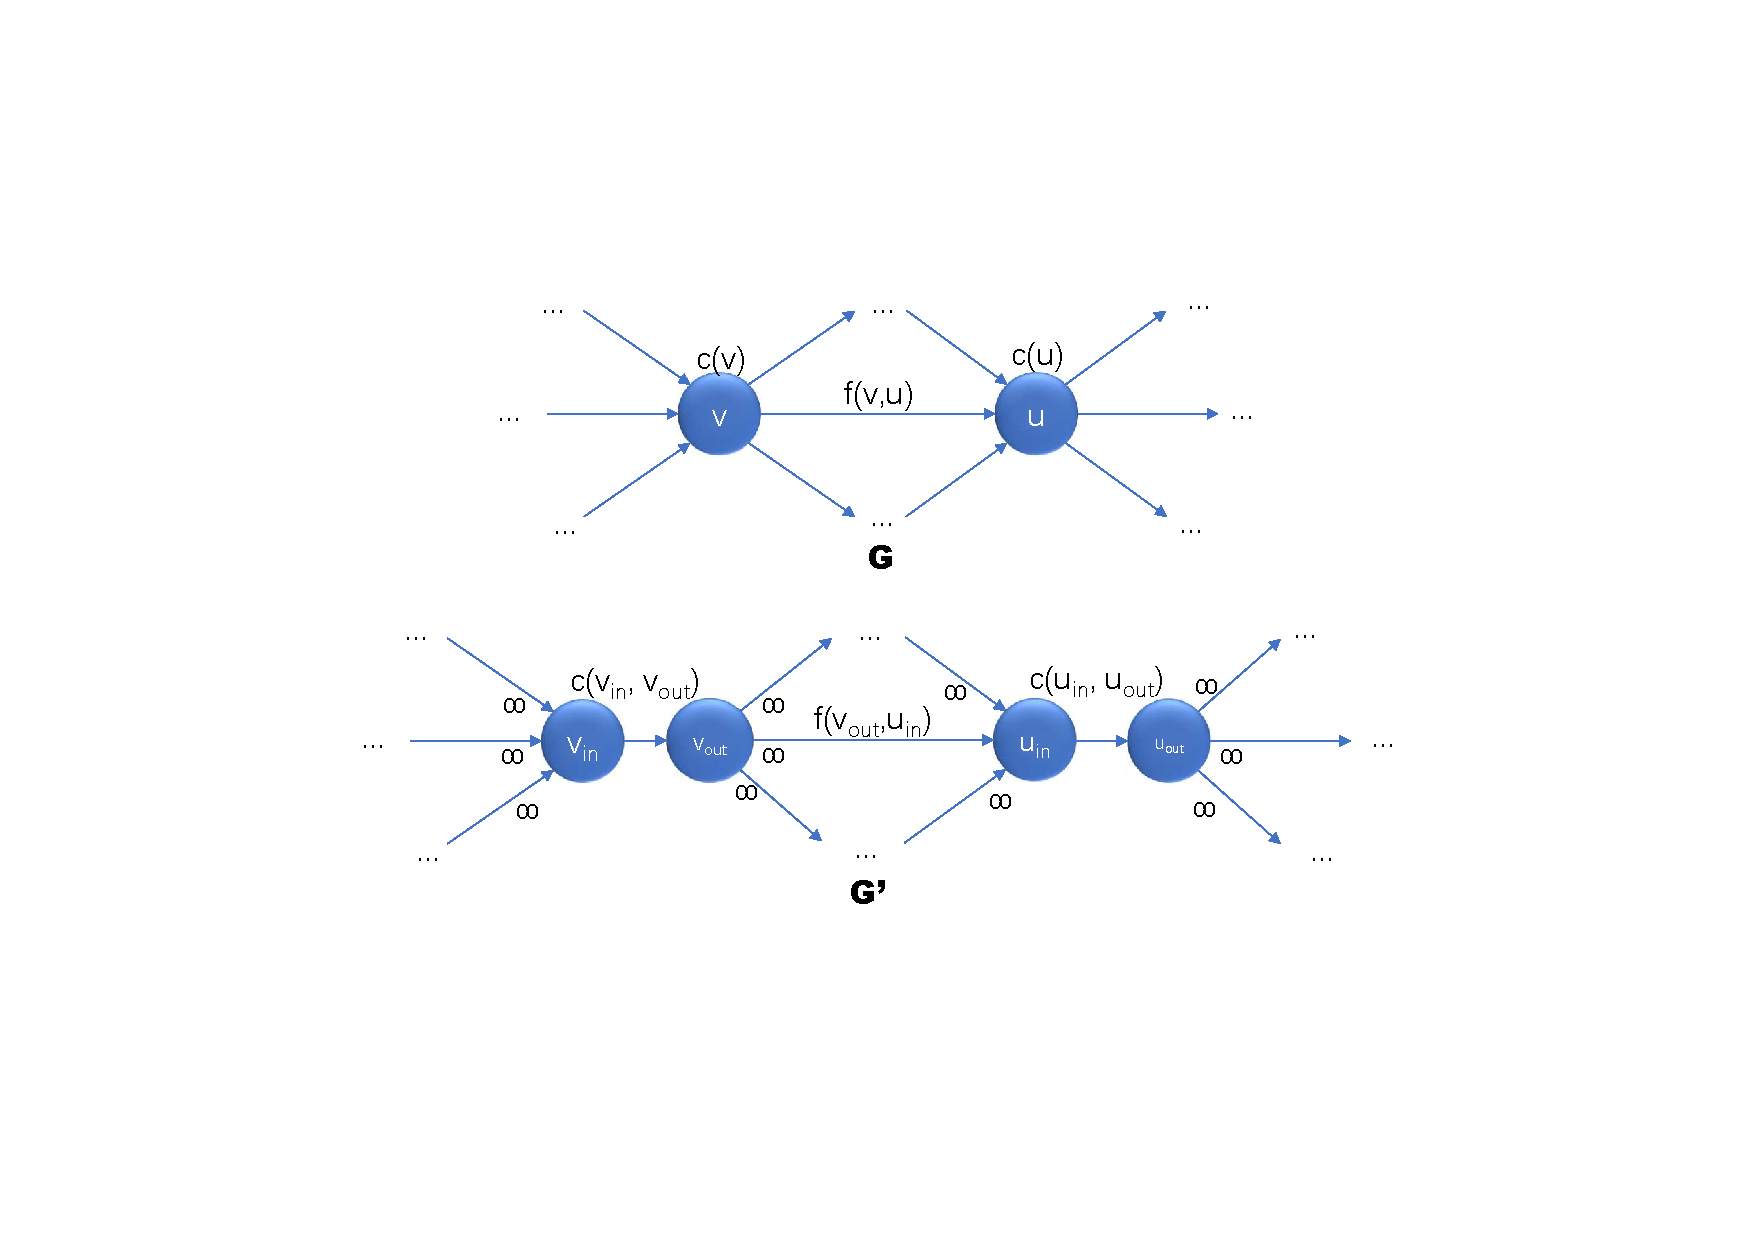
\includegraphics[height=200px]{figures/transform.pdf}
    \caption{An illustration of the transformation}\label{fig-transform}
  \end{figure}
  \item The algorithm requires modification to the original graph $G=(V,E)$. And it is similar to the process we transform the network with vertex capacities into a new net work with edge capacities.
  
  First, for each $v\in V$, split it into two vertices, $v_{in}$ and $v_{out}$ and add an edge $(v_{in},v_{out})$ with capacity 1. Then for each $(u,v)\in E$, convert it into $(u_{out},v_{in})$ with also capacity 1. Then we run Ford-Fulkerson or Edmonds-karp to compute ths max $s-t$ flow. If the result is greater than or equal to $k$, the original answer is yes, there are $k$ internally vertex disjoint paths from $s$ to $t$ in $G$. Else the answer is no. See the pseudo code in Algorithm~\ref{alg:vdp}.
  \begin{algorithm}[H]
    \caption{Algorithm to check whether $k$ internally vertex disjoint $s-t$ paths exist}\label{alg:vdp}
    \begin{algorithmic}[1]
    \Procedure{$k$ vertex-disjoint $s-t$ paths}{$G=(V, E), s, t\in V $}
    \State Create a new empty graph $G'=(V',E')$
    \ForAll{vertex $v\in V$} 
      \State $V'\leftarrow V'\cup \{v_{in},v_{out}\}$
      \State $E'\leftarrow E'\cup \{(v_{in},v_{out})\}$
      \State $c(v_{in},v_{out})=1$
    \EndFor
       \ForAll{edge $(u,v)\in E$ } 
         \State $E'\leftarrow E'\cup \{(u_{out},v_{in})\}$
         \State $c(u_{out},v_{in})=1$
       \EndFor
    \State Compute max $s_{out}-t_{in}$ flow in $G'$, save result as $f$
    \If{$f\geq k$} 
   \State \Return True
   \Else
   \State \Return False
   \EndIf
   \EndProcedure
\end{algorithmic}
 \end{algorithm}
For the construction of the new graph $G'$, the time complexity is O($|V|+|E|$). For computing the max flow, it cost polynomial time. Thus in all this is a polynomial time algorithm.

For correctness of this algorithm, it is easy to see that one unit of flow in $G'$ corresponds to a path in $G$. Since the capacity between $(v_{in},v_{out})$ is restricted to 1, for each pair of two vertices, it is crossed by at most one unit of flow, which corresponds to that in the original graph, no vertex is shared by two paths. Therefore the value of max flow in $G'$ equals to the number of internally vertex disjoint paths in $G$, w.r.t $s,t$.
\end{enumerate}
\begin{exercise} 
  Let $H_n$ be the $n$-dimensional Hamming cube. For $i < n/2$ consider
  $L_i$ and $L_{n-i}$. Note that 
  $|L_i| = {n \choose i} = { n \choose n-i}  = L_{n-i}$, so the 
  $L_i$ and $L_{n-i}$ have the same size.   Show that there are ${n \choose i}$ paths $p_1,p_2,\dots,p_{ {n \choose i}}$
  in $H_n$ such that
  (i) each path $p$ starts in $L_i$ and ends in $L_{n-i}$;
  (ii) two different paths $p,p'$ do not share any vertices.
\end{exercise}
\textbf{Proof.} We can extract all vertices and edges between (including) $L_i$ and $L_{n-i}$, and additionally add a source $s$ and a sink $t$, connect all vertices in $L_i$ to $s$ and all vertices in $L_{n-i}$ to $t$, to form a new graph $G$, where all vertices have capacity 1 except for $s,t$. 

According to our statement in 11.4, if the maximum $s-t$ flow in the new graph is exactly ${n \choose i}$, then there exists ${n \choose i}$ internally vertex disjoint $s-t$ paths in that graph. Further, since all such paths are vertex disjoint, this would mean that in $H_n$, correspondingly each path starts in $L_i$ and ends in $L_{n-i}$, with no vertex shared by two paths.

Remember in 11.1 we proved that the bipartite graph $H_n [L_k \cup L_{k+1}]$ has a matching of size $|L_k| = {n \choose k}$ for $0 \leq k < n/2$, which is a perfect matching since all vertices are covered. From antoher point of view, this tells us that the max flow between $L_k$ and $L_{k+1}$ with respect to vertex capacities is $|L_k|$. With $k$ becoming closer to $n/2$, $|L_k| = {n \choose k}$ monotonically increases, and max flow between two layers increases. For $k>n/2$, the case is symmetric as $n-k<n/2$, $L_{n-k}=L_k={n \choose k}$. 

Therefore the minimum max flow between two adjacent layers in $G$ is $|L_i|=|L_{n-i}|={n \choose i}$, and flow between nonadjacent layers is 0, which restircts the max $s-t$ flow in $G$ to be exactly ${n \choose i}$.\qed

\subsection{Always, Sometimes, or Never Full}


Let $(G,s,t,c)$ be a flow network, $G = (V,E)$. A directed edge $e=(u,v)$ is called always full if $f(e) = c(e)$ for every maximum flow; it is called sometimes full if $f(e) = c(e)$ for some but not all maximum flows; it is called never full if $f(e) < c(e)$ for all maximum flows.

Let $(S, V\setminus S)$ be a cut. That is, $s \in S, t \in V \setminus S$. We say the edge $e = (u,v)$ is crossing the cut if $u \in S$ and $v \in V \setminus S$. We say $e$ is always crossing if it crosses every minimum cut; sometimes crossing if it crosses some, but not all minimum cuts; never crossing if it crosses no minimum cut. For example, look at this flow network:
\begin{center}
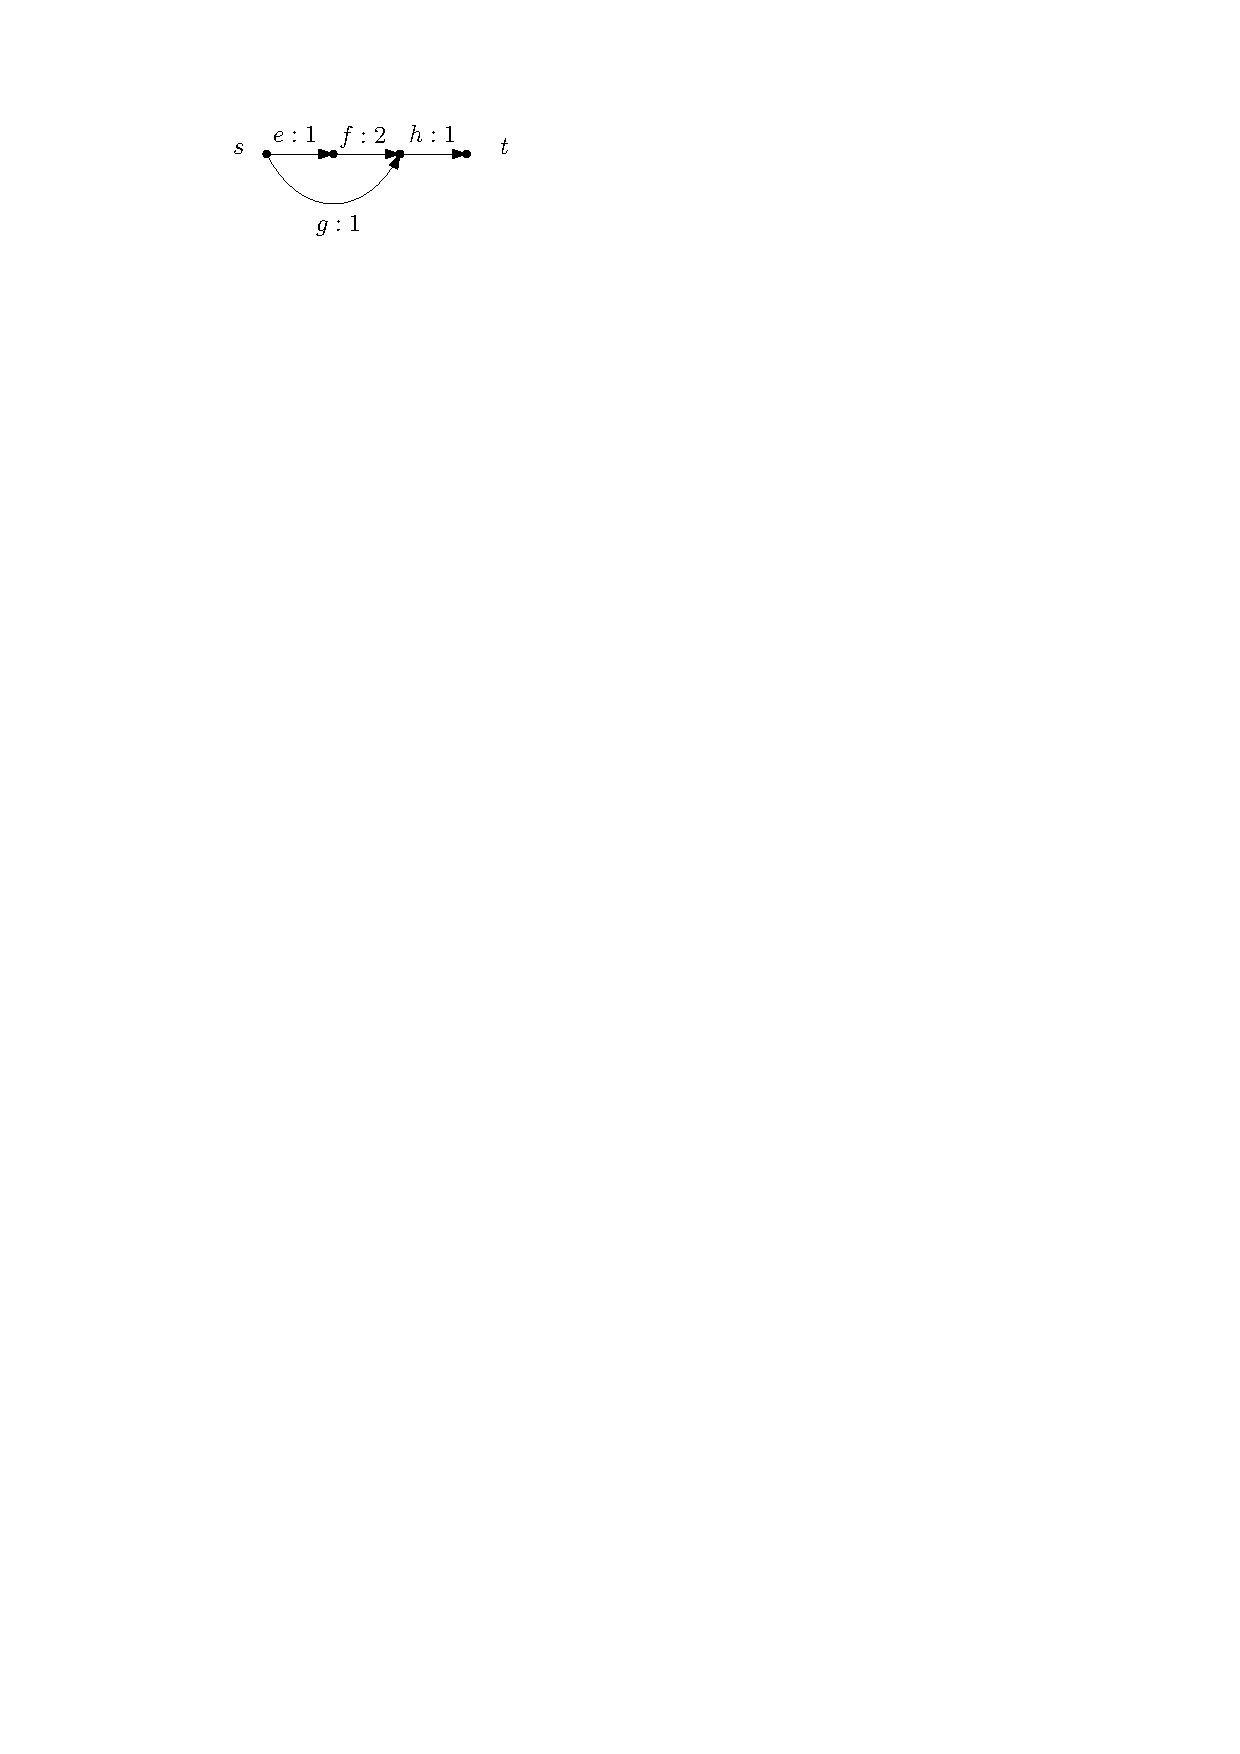
\includegraphics[width=0.4\textwidth]{figures/flow-network-always-sometimes-never.pdf}\\
\small Example network: the edges $e,g$ are sometimes full and never crossing; $f$ is never full and never crossing; $h$ is always full and always crossing.
\end{center}

\begin{exercise}
Consider this network: 
\begin{center}
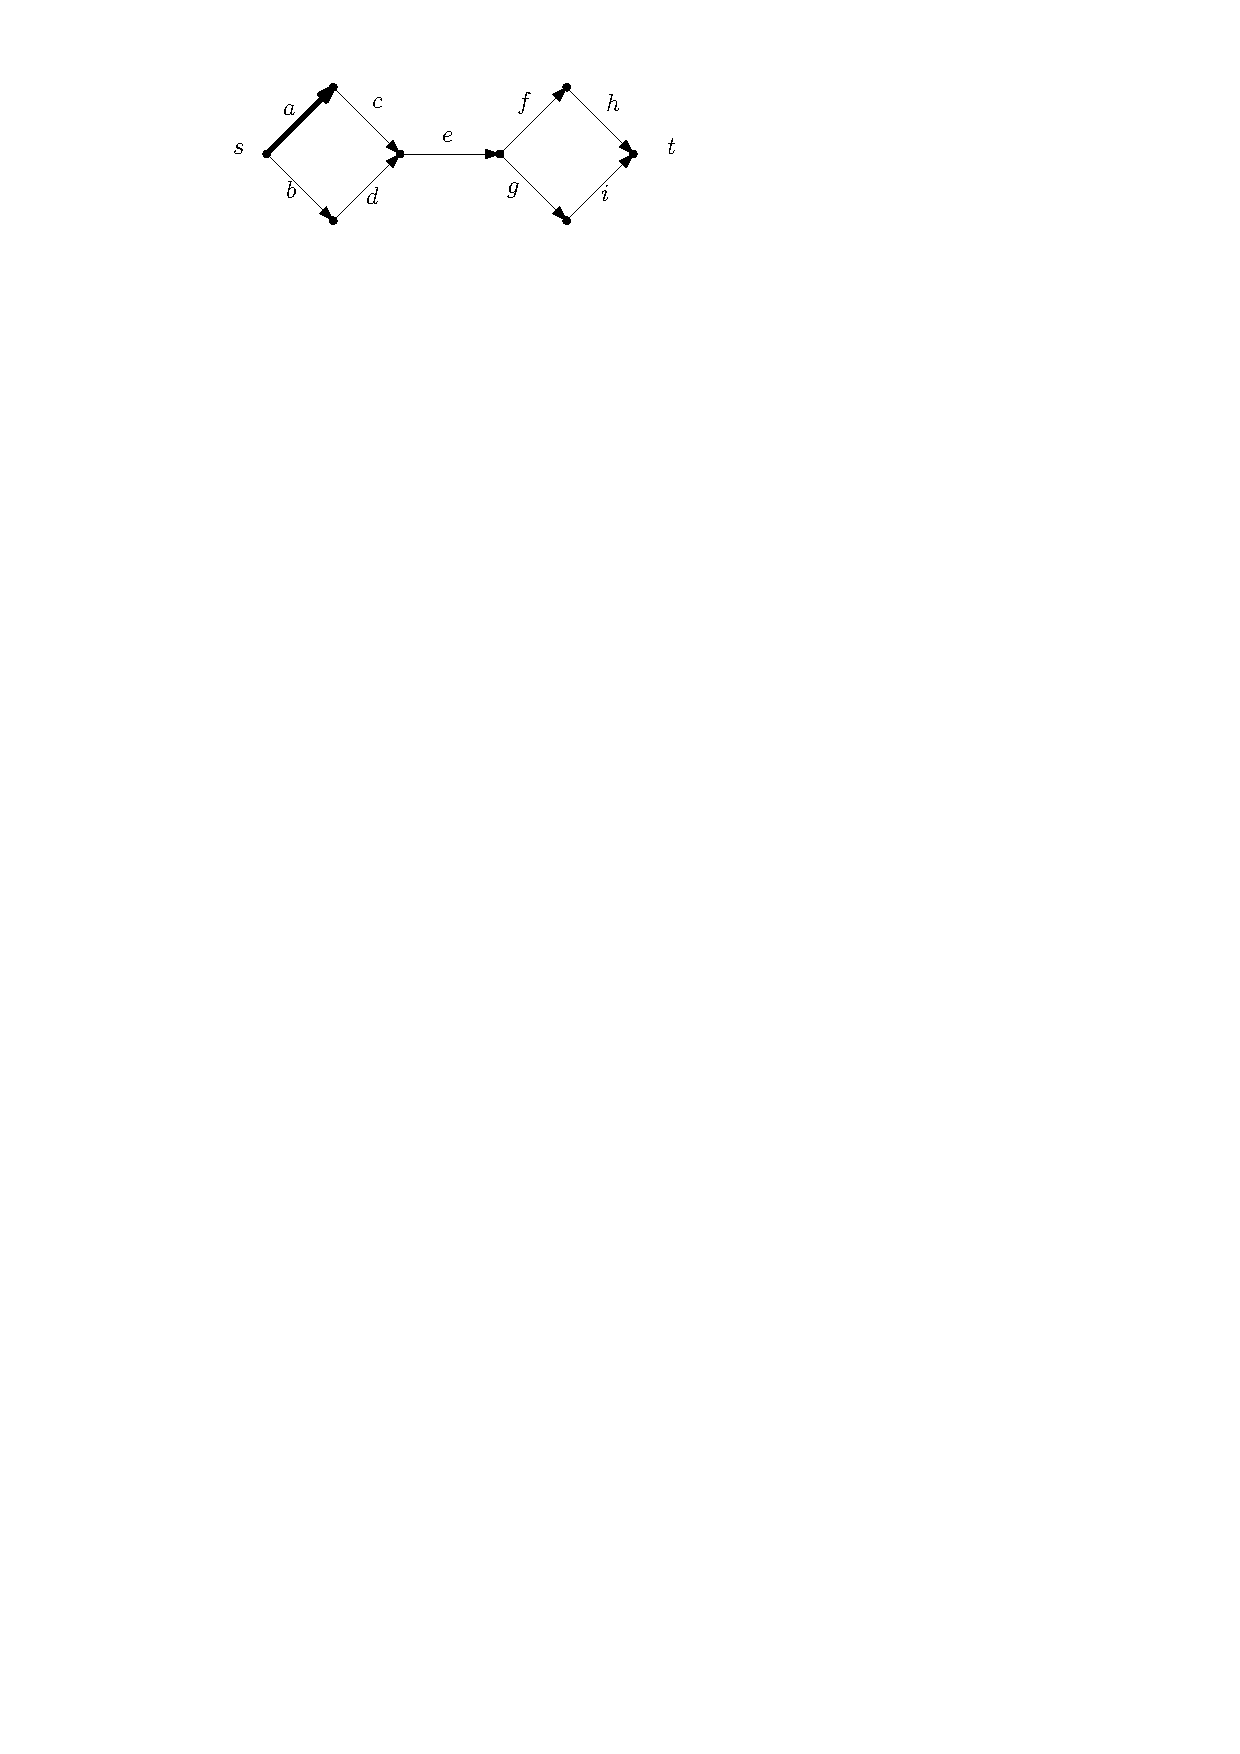
\includegraphics[width=0.6\textwidth]{figures/other-flow-network-always-sometimes-never.pdf}\\
\small The fat edge $a$ has capcity $2$, all other edges have capacity $1$.
\end{center}
\begin{enumerate}
\item Indicate which edges are (i) always full, (ii) sometimes full, (iii) never full.
\item Indicate which edges are (i) always crossing, (ii) sometimes crossing, (iii) never crossing.
\end{enumerate}
\end{exercise}

\begin{proof}
  \begin{enumerate}
    \item
    Always full: $e$\par
    Sometimes full: $b,c,d,f,g,h,i$\par
    Never full: $a$\par

    \item
    Always crossing: $e$\par
    Somtimes crossing: no one\par
    Never crossing: $a,b,c,d,f,g,h,i$\par

  \end{enumerate}
\end{proof}

\begin{exercise}
An edge $e$ can be ($x$) always full, ($y$) sometimes full, ($z$) never full; it can be ($x$') always crossing, ($y'$) sometimes crossing, ($z'$) never crossing. So there are nine possible combinations: ($xx'$) always full and always crossing, ($xy'$) always full and sometimes crossing, and so on. Or are there? Maybe some possibilities are impossible. 
Let's draw a table:
\begin{center}
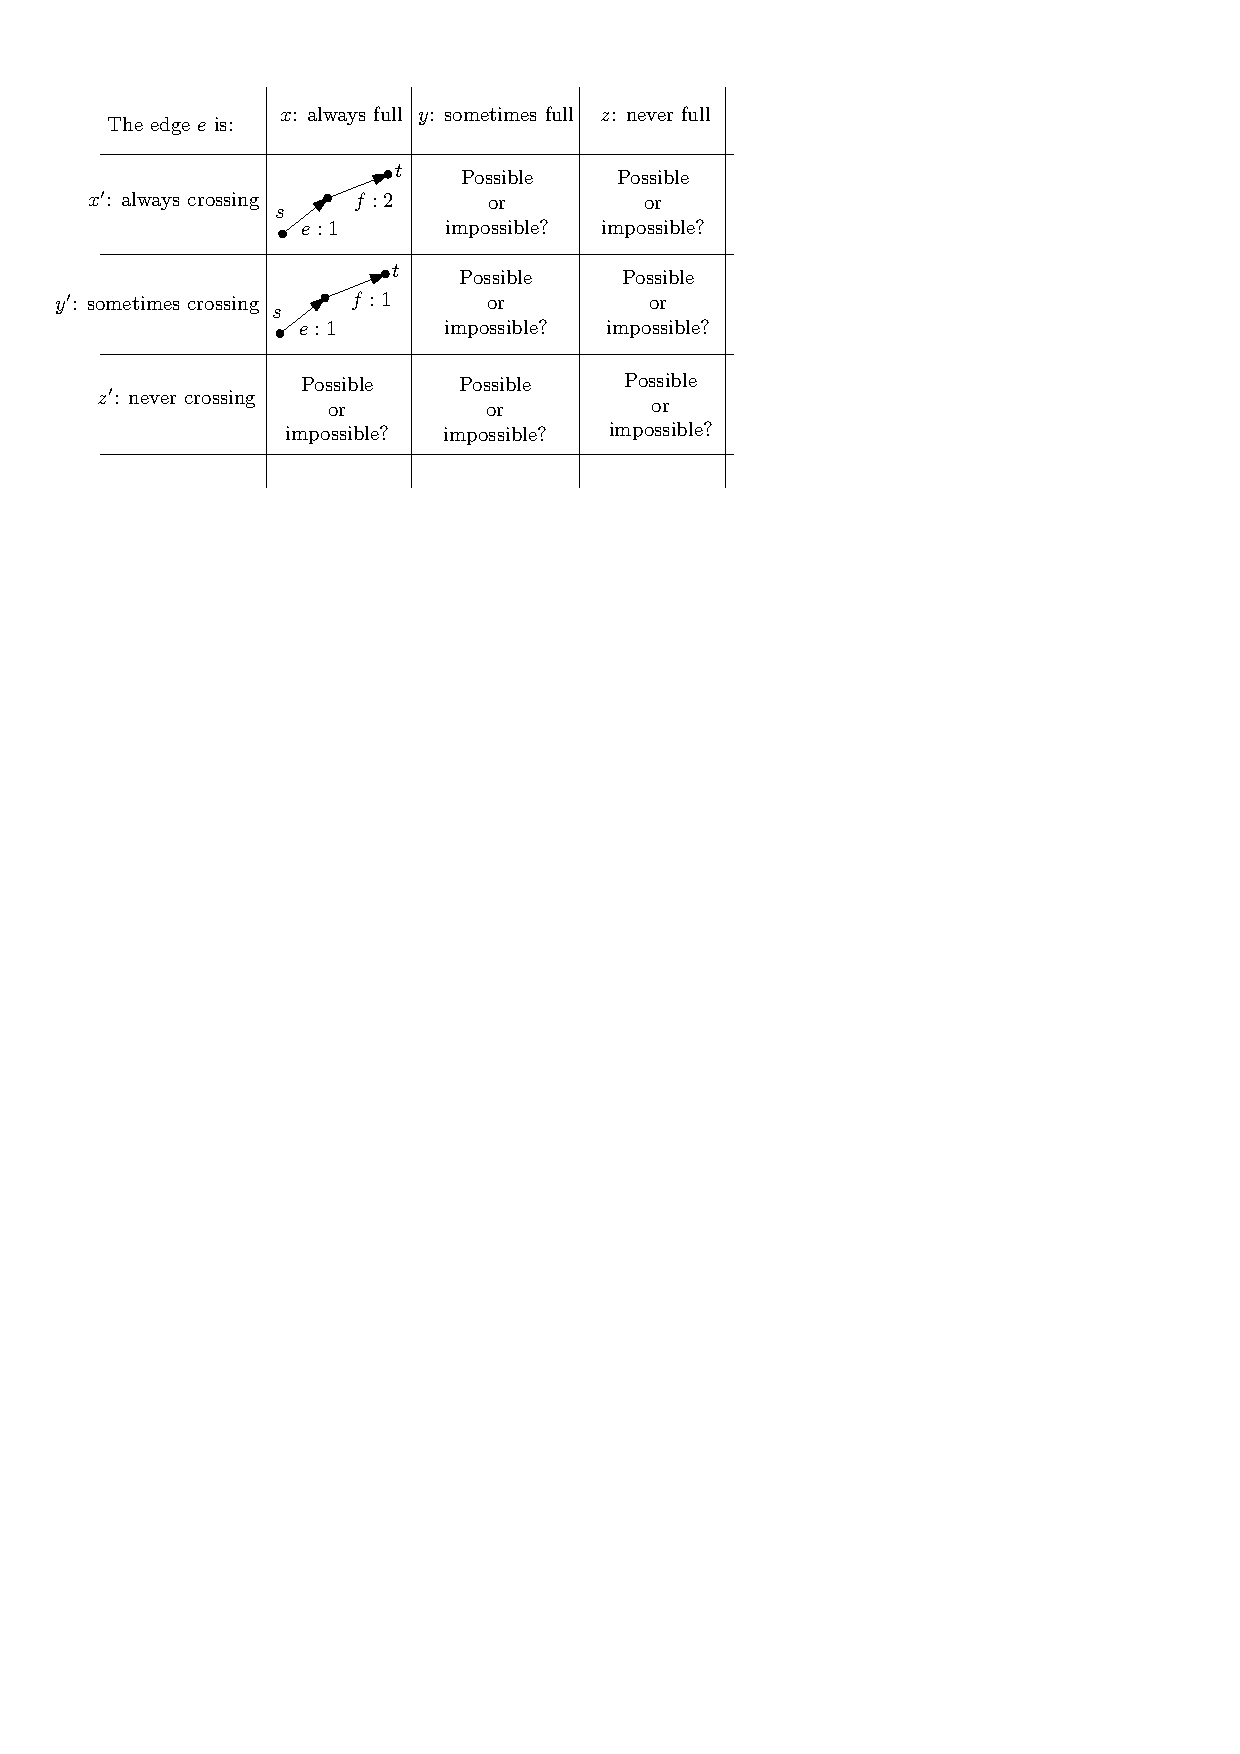
\includegraphics[width=0.8\textwidth]{figures/always-somtimes-never-table.pdf} \\
\small The nine possible cases, some of which are maybe impossible.
\end{center}
The two very simple flow networks in the table already show that $(xx')$ and $(yy')$ are possible; that is,
it is possible to be always full and always crossing, and it is possible to be always full and sometimes crossing.
Fill out the table! That is, for each of the remaining seven cases, find out whether it is possible or not. If it is
possible, draw a (simple) network showing that it is possible; if impossible, give a proof of this fact.
\end{exercise}

\begin{proof}

  $(xz')$ is impossible. Since the maximum flow equals to the minimum cut, if an edge is always full then it is possible to be part of some minimum cut.\par
  $(yx')$ and $(yy')$ are impossible. If a network has several different minimum cut, then the edges in these minimum cut should be full in the maximum flow.\par
  $(zx')$ and $(zy')$ are impossible. By the definition, if an edge is not full, it cannot be a part of the minimum cut.\par
  \begin{figure}[htbp]
  \begin{center}
  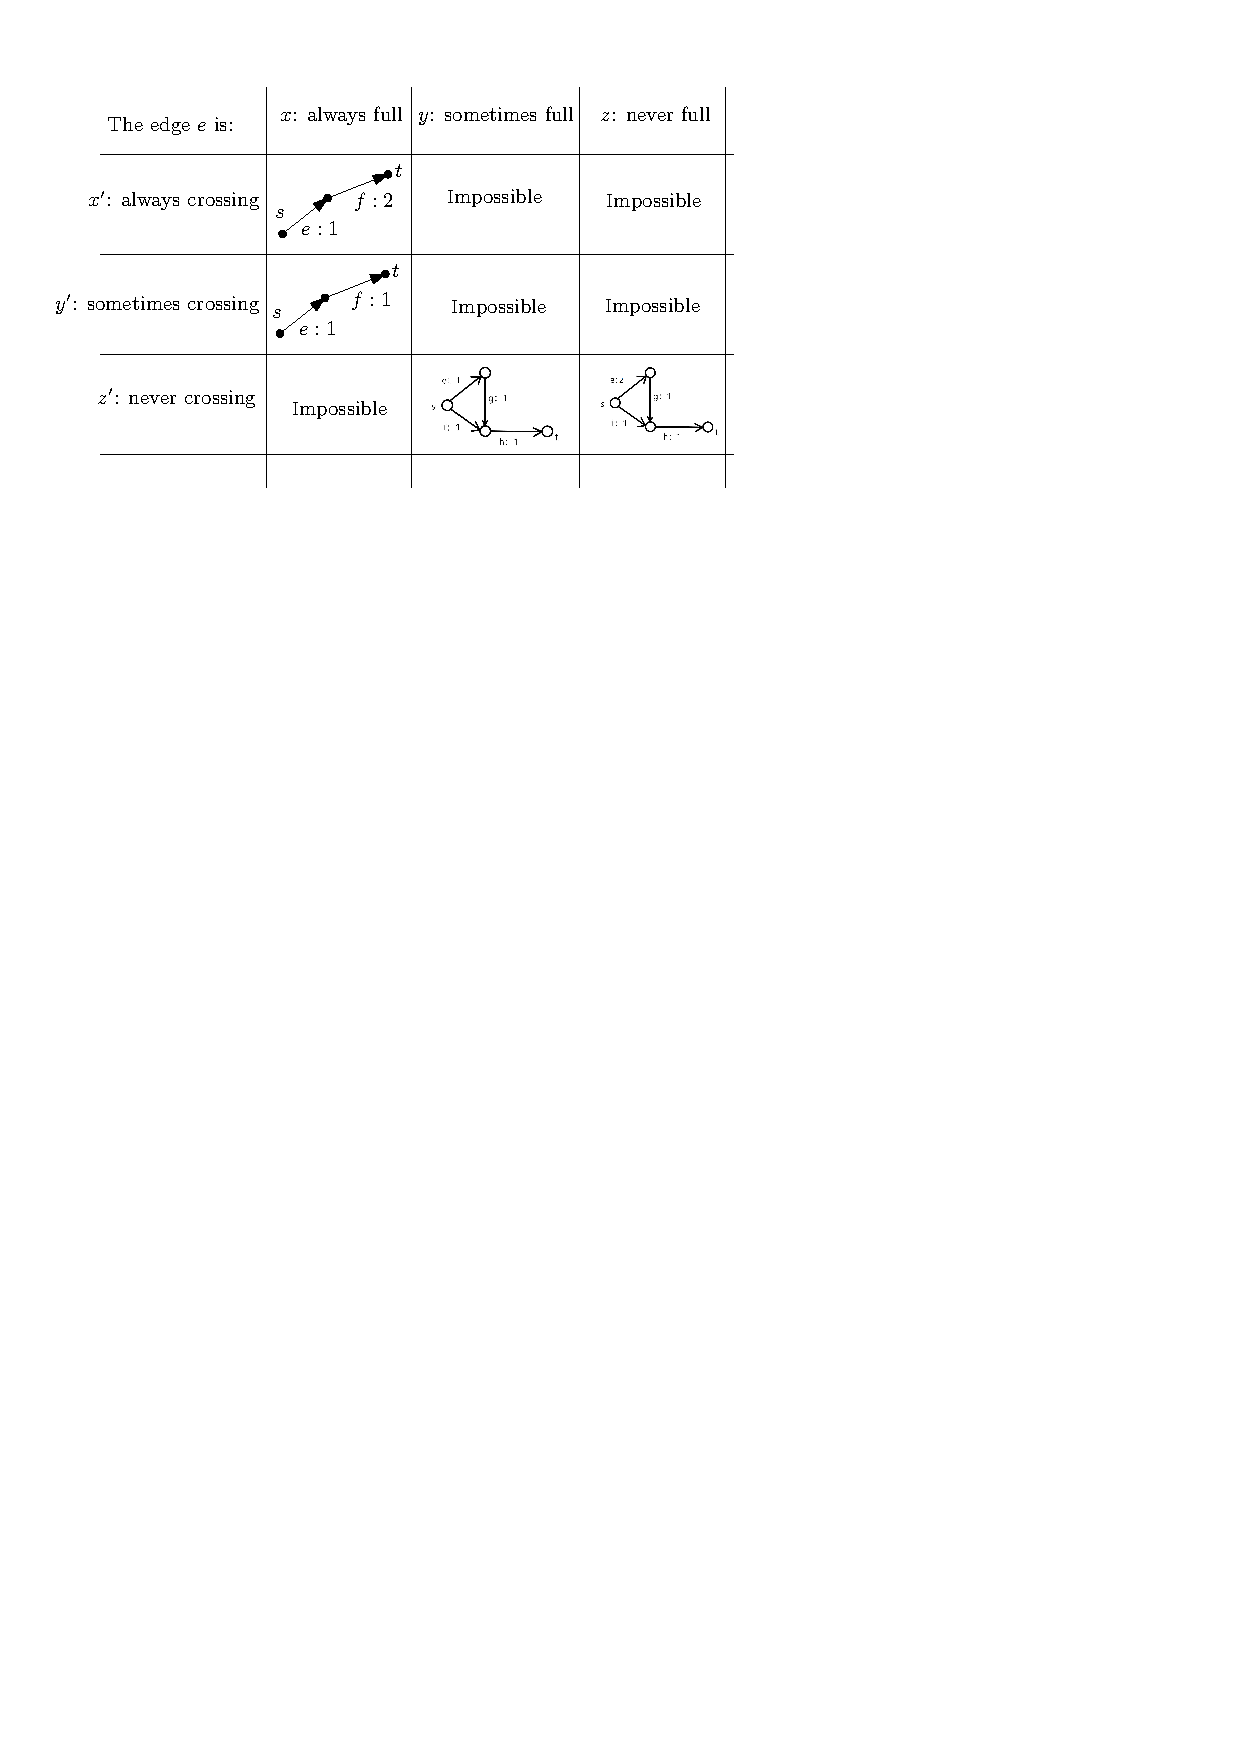
\includegraphics[width=0.8\textwidth]{figures/always-somtimes-never-table-answer.pdf}

  \end{center}
\end{figure}
\end{proof}

\subsection{Multi-Commodity Flow}

In class, we discussed the Multi-Commodity Flow problem. Formally, a multi-commodity network is 
given by a directed graph $G = (V,E)$, a capacity function $c: E \rightarrow \R^+$, and 
sources $\vec{s} = (s_1,\dots,s_k)$ and sinks $\vec{t} = (t_1,\dots,t_k)$ in $V$.
A {\em multi-commodity flow} in $(G,c,\vec{s}, \vec{t})$ is a tuple $(f_1,\dots,f_k)$ 
where each $f_i$ is an $s_i$-$t_i$-flow in $(G,c, s_i, t_i)$, that is, $f_i$ is individually a flow, satisfying 
flow conservation constraints at all vertices except $s_i$ and $t_i$; the {\em value} of $f_i$, $\val(f_i)$,
is the outflow at $s_i$, as usual. Furthermore,
$ \sum_{i=1}^k f_i(e) \leq c(e)$ for all edges $e \in E$. Think of each $f_i$ as being a way to route
units of good $i$ from $s_i$ to $t_i$. \\

The {\em Maximum Multi-Commodity Flow Problem} (Max-MCF) asks for a multi-commodity flow
in the network maximizing the total value, i.e., $\val(f_1) + \cdots + \val(f_k)$.\\

In the {\em Feasibility Multi-Commodity Flow Problem} (F-MCF), we are additionally given {\em demands}
$d_1,\dots,d_k$, and we want to decide whether there is a multi-commodity flow $(f_1,\dots,f_k)$
with $\val(f_i) = d_i$. If there is such a multi-commodity flow, we say the instance of F-MCF is {\em feasible},
otherwise we say it is {\em infeasible}.

\begin{center}
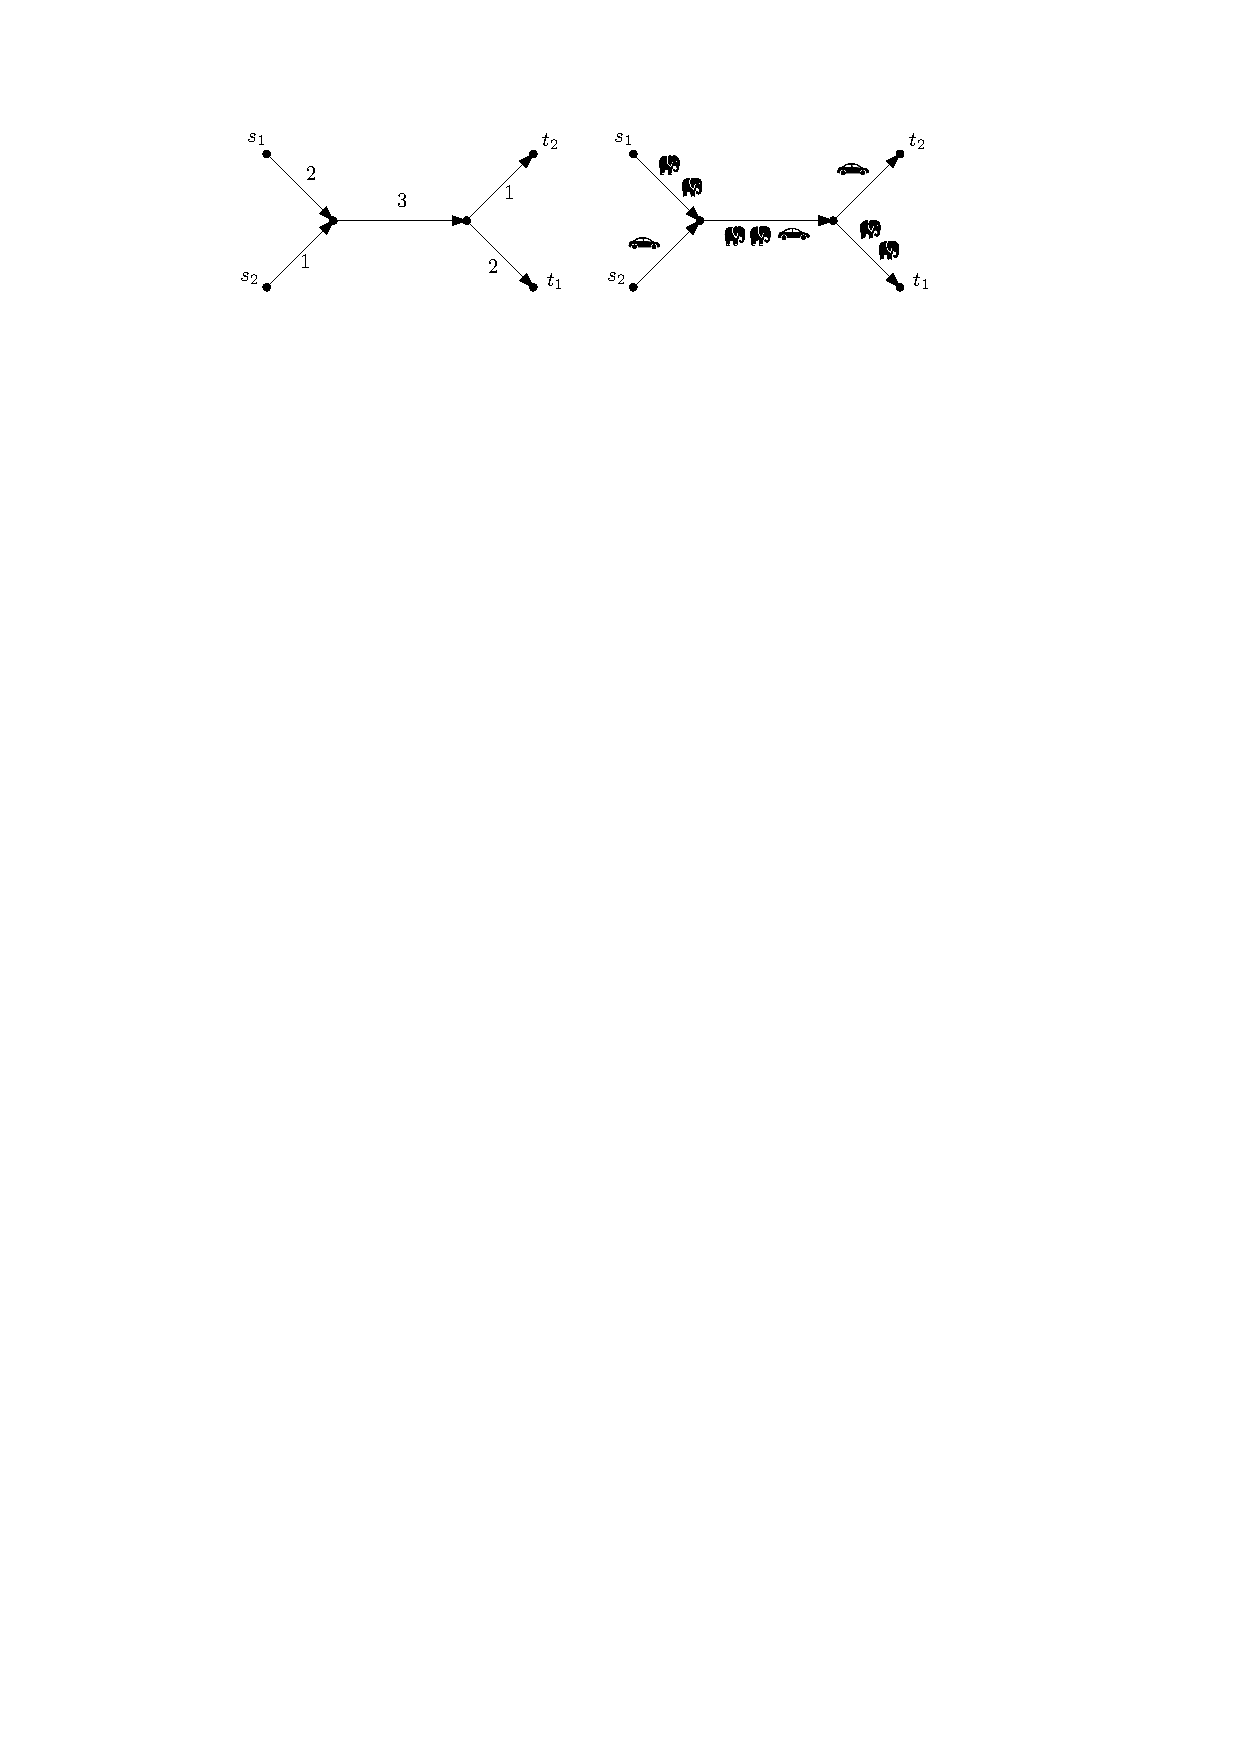
\includegraphics[width=\textwidth]{figures/multi-commodity-flow.pdf}\\
\small A multi-commodity flow routing two elephants from $s_1$ to $t_1$ and one car from $s_2$ to $t_2$.
Note that the two flows share the middle edge; also, all flow values and all capacities are integers.
\end{center}

For each of Max-MCF and F-MCF we can define the {\em integer} version: Max-IMCF and F-IMCF.
These are the same problems as above, but we additionally require that all capacities, demands, and
flow values be integers.

\begin{exercise}
    Find a multi-commodity flow network with integer capacities such that Max-MCF is larger than
    Max-IMCF. That is, to achieve the maximum possible flow, it is necessary to use non-integral flows.
\end{exercise}

\begin{proof}
	All capacities are 1. All demands are 1, too. The Max Commodity Flow is 1.5.
\begin{figure}[htbp]
  \begin{center}
  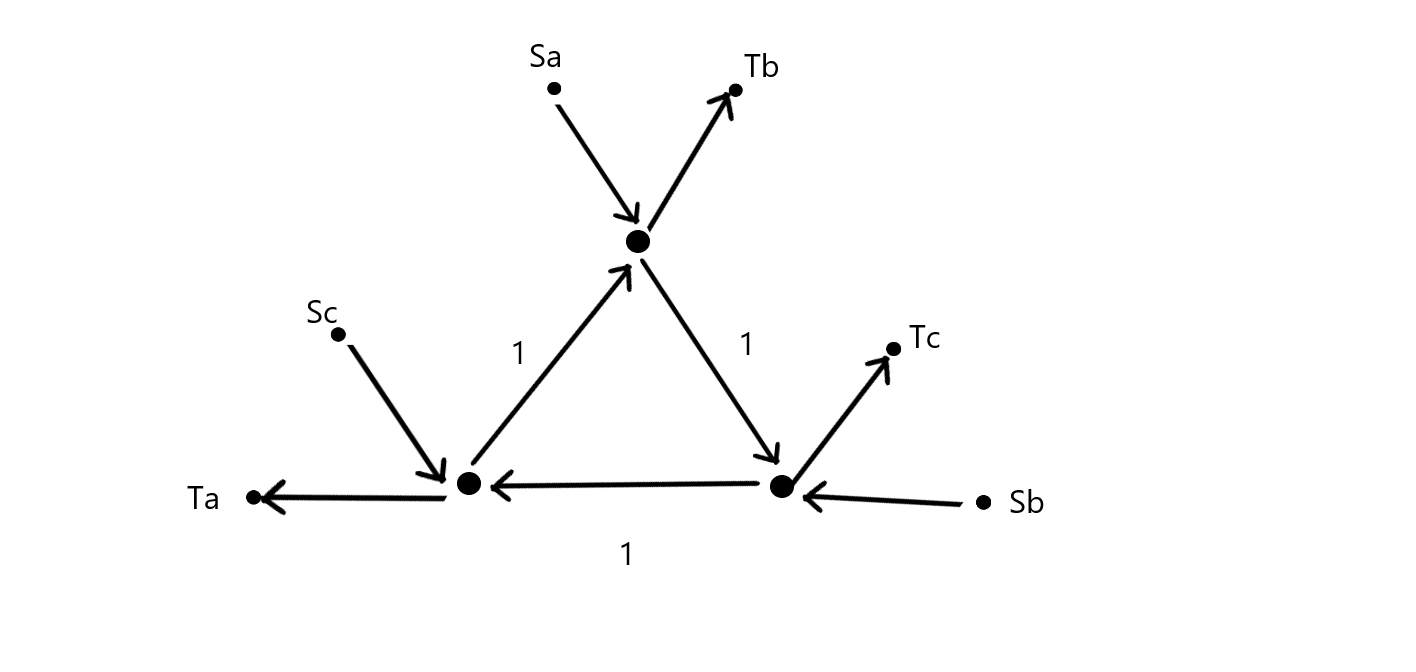
\includegraphics[width=0.8\textwidth]{figures/E11.png}

  \end{center}
\end{figure}
\end{proof}

\begin{exercise}
    Find a multi-commodity flow network with integer capacities and integer demands such that 
    the F-MCF problem is feasible but the F-IMCF problem is infeasible. That is, it is possible
    to satisfy all the demands, but not all flows must be integer.
\end{exercise}


\end{document}
